\chapter{Methodology}
\label{chapter:methodology}

\section{Experimental setup}

The final RRC system is shown as a block diagram in Figure \ref{figure:rrc-block},
and the actual network topology is equivalent to the one in Figure \ref{figure:rbn-reservoir}.

\todo{Her kommer det stort bilde av mitt reservoir-setup med justerbar in- og ut-koblinger}

\todo{gotta add moar stuffz here, nemlig varierende input/output cocnnectivitet støtte}

\begin{figure}
    \centering
    \begin{tikzpicture}
        \node (dataset) {Dataset};
        \node[box, below=of dataset] (input) {Input layer};
        \node[box, right=of input] (reservoir) {RBN Reservoir};
        \node[box, right=of reservoir] (readout) {Readout layer};
        \node[above=of readout] (classification) {Classification};

        \node[draw,dotted,fit=(input) (reservoir) (readout), label={RRC}] {};

        \draw[edge] (dataset) to (input);
        \draw[edge] (input) to (reservoir);
        \draw[edge] (reservoir) to (readout);
        \draw[edge] (readout) to (classification);
    \end{tikzpicture}
    \caption{Block diagram of the RRC processing a dataset.}
    \label{figure:rrc-block}
\end{figure}

\subsection{testing}

To verify that RBN simulation is working,
a RBN is created randomly, initial state set to all zeros, and ran.
The results are visualized in Figure \ref{figure:rbn-noperturb}.
We see that the RBN exhibits stable dynamics, and enters into an attractor around $t=15$.
In Figure \ref{figure:rbn-perturb} we continiously perturb the RBN with the input stream from the Temporal Parity task visualized in Figure \ref{figure:temporal-parity}.
In the perturbed case, the state trajectory is continiously changed, preventing the RBN from settling into an attractor.
Interestingly enough, there seems to be a visual similarity between the two cases.
Such a pattern is sure to dissapear with a RBN in the chaotic phase.

This erratic pattern of state transitions is then fed into the readout layer,
which is then tasked with finding a linear combination of the RBN states that results in the expected output for the given task.

\begin{figure}
  \subfloat[Unperturbed]{
    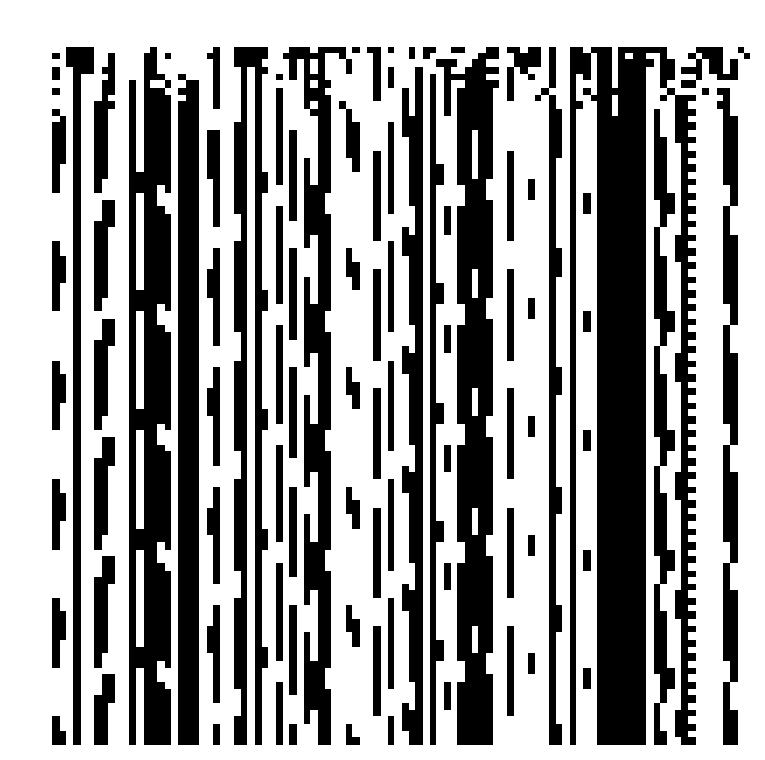
\includegraphics[width=0.5\columnwidth]{method/final-1-noperturb.pdf}
    \label{figure:rbn-noperturb}
  }
  \subfloat[Perturbed]{
    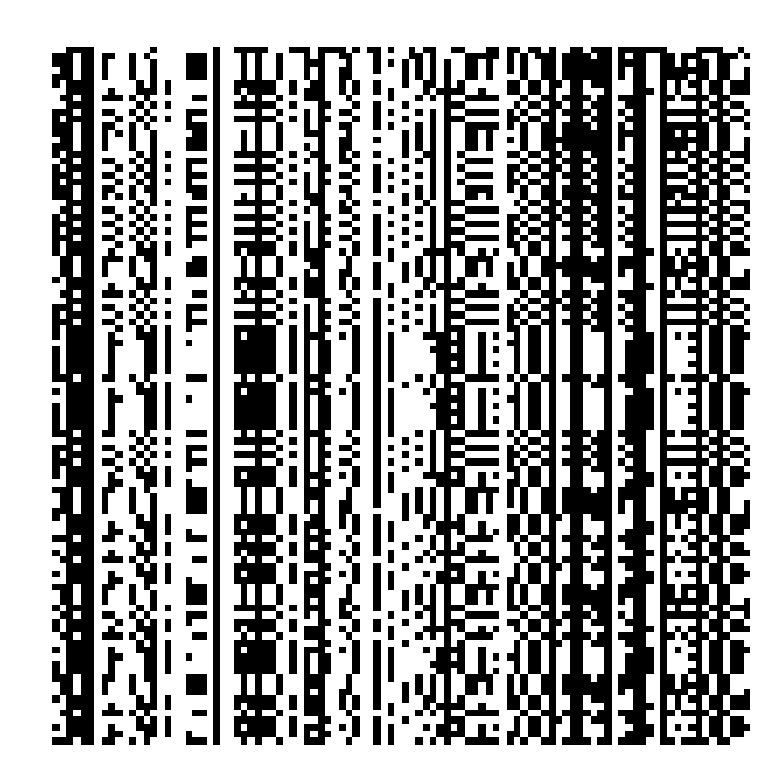
\includegraphics[width=0.5\columnwidth]{method/final-1-perturb.pdf}
    \label{figure:rbn-perturb}
  }
  \caption{
    The same RBN ($N=100, K=2, P=0.5, L=50$) shown both perturbed and unperturbed.
    The boolean states of the RBN are plotted along the X-axis,
    with time flowing downwards.
  }
\end{figure}

\subsection{Training}

To train the RRC system we require large training datasets,
as well as different, smaller datasets for testing the trained system.
We will use the datasets described in section \ref{subsection:rbn-reservoir-systems}.

We then either create a new RBN (initialize it randomly),
or load a previously created RBN from disk.
For each bit of input in each dataset,
we perturb the input-connected nodes in the RBN.
After each perturbance, the RBN is ran synchronously (CRBN mode) for one timestep.
The resulting RBN states are collected,
and after the entire dataset is processed,
forwarded to the readout layer.

To find a suitable mapping from the set of reservoir states and the correct input classification,
ridge regression \cite{hoerl1970ridge} is used.
This version of least squares regression is more accurate when faced with input colinearities, as well as always being at least as accurate as ordinary least squares.  
This process is repeated for all the datasets,
and the final regression parameters are chosen as a combination of the parameters obtained for each individual dataset.
Finally we measure the normalized accuracy of the trained reservoir on the test dataset,
defined as the following:
\begin{equation}
Accuracy = 1 - \dfrac{sum(actual\_output \neq expected\_output)}{len(correct\_output)}
\label{formula:accuracy}
\end{equation}

\subsection{Attractor analysis}

\todo{Should i present the theory on attractor analysis here instead of inline in section \ref{section:reservoir-dynamics}}?
